\chapter{Zásuvný modul pro QGIS}
\label{6-plugin}

\section{Tvorba QGIS zásuvného modulu}
\label{plugin-tvorba}

Do projektu Quantum GIS je možné psát zásuvné moduly v~jazycích C++ nebo Python.
Dnes už jsou častější zásuvné moduly psané v~Pythonu, přesto se však objevují
i~ty v~C++, a~to z následujících důvodů. QGIS jako takový je napsán v~tomto 
jazyce. Jedná se o~objektově orientovaný jazyk, hodí se proto pro větší projekty. 
Nevýhodou C++ pluginů je nutnost kompilace, kterou však vyváží výsledná větší 
rychlost běhu aplikace.V~případě zásuvného modulu \textit{Conflate} byl jazyk 
C++ zvolen i~z~důvodu použití knihovny \textit{GEOS}, která je psána rovněž 
v~tomto jazyce.

% zmínka o licenci? Vzhledem k tomu, že C++ pluginy většinou využívají knihovny
% libqgis*.so, které jsou publikovány pod licencí GNU GPL, musí být tyto
% moduly pod stejnou licencí.

C++ zásuvné moduly QGISu jsou dynamické knihovny (\textit{.so} nebo 
\textit{.dll} \footnote{ přípona \textit{.so} se používá v~Linuxu, přípona 
\textit{.dll} pod systémem Windows}). Načtení modulu v~QGISu probíhá za~běhu 
programu. Při startu programu \textit{Správce zásuvných modulů 
(Plugin Manager)} vyhledá všechny soubory s~danou příponou ve~složce 
se~zásuvnými moduly (v Linuxu nejčastěji /lib/qgis nebo 
/usr/lib/qgis/plugins), popřípadě v~dalších složkách, jejichž umístění
je definováno v~uživatelském nastavení, a~načte je.

Pro správné načtení musí zásuvný modul obsahovat následující.

\begin{enumerate}
 \item Funkce \texttt{classFactory()}, která vytvoří instanci daného pluginu.
 \item Metoda \texttt{initGui()}, jejímž prostřednictvím jsou zobrazeny prvky 
	uživatelského rozhraní (ikona apod.) v~nabídce \textit{Zásuvné moduly 
	(Plugins)} a~v~liště nástrojů.
 \item Metoda \texttt{unload()}, která odstraní alokované elementy a~samotnou
	instanci třídy zásuvného modulu (pomocí destruktoru) při ukončení 
	programu.
 \item Další externí C ~funkce (\texttt{na\-me(), descrip\-tion()}) pro správné
	zobrazení ve~\textit{Správci zásuvný modulů}.
\end{enumerate}

V~modulu \textit{Conflate} jsou všechny tyto funkce obsaženy ve~třídě
\texttt{Qgs\-Con\-flate\-Plugin}. 
Podrobnější popis tvorby C++ pluginu lze najít v~\textit{QGIS Coding and 
Compilation Guide} % uvést odkaz na literaturu
, odkud byly čerpány výše uvedené informace.


% pro testování konzolová aplikace
% základní informace + zásady


\section{Zásuvný modul \textit{Conflate}}
\label{plugin-navrh}
% návrh gui, funkčnost

Zásuvný modul \textit{Conflate} pro QGIS, který je jedním z~výstupů této práce,
umožňuje spojení vektorových datasetů. Pro tento proces úpravy vrstev využívá
tříd a metod výše popsané knihovny \textit{GEOC}.

Modul se skládá celkem ze~tří tříd \texttt{QgsConflateProvider}, 
\texttt{QgsConflatePlugin} a~ \texttt{QgsDialog}. Třída \texttt{QgsConflatePlugin} 
obsahuje funkce pro vytvoření a~načtení zásuvného modulu do~QGISu tak, jak bylo 
uvedeno v~kapitole \ref{plugin-tvorba}. Zobrazování a~interakci s~uživatelem 
zajišťuje třída \texttt{QgsDialog}. Konečně třída \texttt{QgsConflateProvider} 
se stará o~funkcionalitu aplikace a~obsahuje tak funkce využívající knihovnu 
\textit{GEOC} i~další funkce pro kopírování vrstvy, změnu geometrie, výpis 
protokolu apod.

\vspace{0.5cm}
\label{schema}
  \begin{figure}[h]
    \centering
      \input{./pictures/schema.pdf_tex}
      %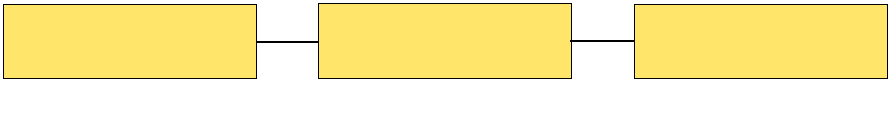
\includegraphics[width=350pt]{./pictures/schema.pdf}
      \caption{Architektura zásuvného modulu \textit{Conflate}}
      \label{fig:schema}
  \end{figure} 

%Grafické rozhraní je navrženo tak, aby splňovalo zásady tvorby uživatelského
%rozhraní dle ... % odkaz na literaturu. ...
%Vzhled dialogu byl vytvořen pomocí nástroje QT Designer.

Následuje výčet činností probíhajících při spuštění a~použití \textit{Conflate}.
Tento výčet má za~úkol pouze zprostředkovat čtenáři představu, jak modul funguje.
Podrobný návod pro jeho použití z~hlediska uživatele je pak rozepsán v~příloze
v~uživatelské příručce. Popis jednotlivých metod zas lze nalézt v~anglické
dokumentaci k~pluginu. % doplnit odkazy na přílohy

\begin{enumerate}
 \item Při otevření dialogu se do~rozbalovací nabídky načtou názvy vrstev 
	otevřených v~programu.
 \item Dalším krokem je výběr vrstev a~nastavení možností uživatelem.
 \item Po~spuštění zpracování se nejdříve zkopíruje upravovaná vrstva 
	(\textit{Subject layer}) do~nové vektorové vrstvy pomocí funkce 
	\texttt{copyLayer()}. Formát nové vrstvy je vždy \textit{shapefile}
	\footnote{ESRI Shapefile je datový formát pro ukládání vektorových 
	  prostorových dat  vyvinutý firmou Esri, jedná se o~jeden 
	  z~nejrozšířenějších formátů dat pro geografické informační systémy,
	  přípona souborů v tomto formátu je .shp}.
	Tato vrstva je vytvořena v~aktuální složce a~její název odpovídá vzoru 
	\begin{center}
	 \texttt{nazev\_puvodni\_vrstvy(nejnizsi\_nepouzite\_cislo).shp},
	\end{center}
	např. \texttt{subject(3).shp}.
 \item Poté je převedena geometrie prvků zvolených vrstev (upravovaná
	a~referenční) na~reprezentaci geometrie knihovny \textit{GEOC},
	tedy z~\texttt{Qgs\-Geo\-metry} na~\texttt{GEOC\-Geo\-metry}. 
	Tyto geometrie 	jsou uloženy do~vektorů, které se pak předají 
	třídám \textit{GEOC}.
 \item Jak už bylo naznačeno, je vytvořena instance příslušné třídy 
	\textit{GEOC} a~té jsou předány parametry - vektory s~prvky vybraných
	vrstev a~toleranční vzdálenost. 
 \item Dále je zavolána funkce vytvořené třídy pro zarovnání datasetů. Při volbě 
	při\-chycení vrcholů \textit{Snap vertices} v~dialogu je použita třída 
	\texttt{Vertex\-Snapper} a~metoda \texttt{snap()}, při volbě zarovnání 
	vrstev \textit{Coverage Alignment} třída \texttt{Cove\-rage\-Align\-ment} 
	a~metoda \texttt{align()}, poslední možností je \textit{Match Lines}, která
	využívá třídu \texttt{Line\-Matcher} a~její metoda \texttt{match()}. 
	Výsledek je uložen do~nového vektoru geometrií.
 \item Na závěr je upravena geometrie nové vrstvy (kopie upravované vrstvy) dle
	výsledků úprav provedených algoritmy knihovny \textit{GEOC}.
 \item Nová vrstva se automaticky přidá do~aktuálního projektu v~QGISu a~zobrazí
	se v~panelu \textit{Vrstvy (Layers)}.
 \item Po~zpracování vrstvy se do textového okna dialogu vypíše protokol 
	o~zpracování, který obsahuje název vstupních a~výstupních dat, počet
	zpracovácaných prvků a~počet nevalidních prvků včetně výpisu jejich
	identifikátorů (\textit{id}).
\end{enumerate}


\section{Ukázky}
\label{plugin-ukazky}
% obrázky s popisem funkcionality





 

